%
% File emnlp2018.tex
%
%% Based on the style files for EMNLP 2018, which were
%% Based on the style files for ACL 2018, which were
%% Based on the style files for ACL-2015, with some improvements
%%  taken from the NAACL-2016 style
%% Based on the style files for ACL-2014, which were, in turn,
%% based on ACL-2013, ACL-2012, ACL-2011, ACL-2010, ACL-IJCNLP-2009,
%% EACL-2009, IJCNLP-2008...
%% Based on the style files for EACL 2006 by 
%%e.agirre@ehu.es or Sergi.Balari@uab.es
%% and that of ACL 08 by Joakim Nivre and Noah Smith

\documentclass[11pt,a4paper]{article}
\usepackage[hyperref]{emnlp2018}
\usepackage{times}
\usepackage{latexsym}
\usepackage{url}

% self added
\usepackage{graphicx}
\usepackage{amsmath}
\usepackage{multirow}
\usepackage{xspace}
\usepackage{bm}
\usepackage{amssymb}
\usepackage{booktabs}
\usepackage{pgfplots}


\newcommand{\etal}{et al.\xspace}
\newcommand{\eg}{e.g.\ }
\newcommand{\ie}{i.e.\ }
\newcommand{\etc}{etc.\ }

\newcommand{\system}[2][]{\texttt{#2#1}\xspace}
\newcommand{\class}[2][]{\texttt{#2}#1\xspace}

\newcommand{\secref}[1]{Section~\ref{#1}\xspace}
\newcommand{\tabref}[2][]{Table#1~\ref{#2}\xspace}
\newcommand{\figref}[2][]{Figure#1~\ref{#2}\xspace}
\newcommand{\exref}[2][]{Example#1~(\ref{#2})\xspace}
\newcommand{\equref}[2][]{Equation#1~\ref{#2}}
\newcommand{\bracketref}[1]{(\ref{#1})\xspace}

\newcommand{\myparagraph}[1]{\noindent{\textbf{#1}}~}
%\newcommand{\myparagraph}[1]{\paragraph{#1}}

\newcommand{\bb}[1]{\mathbb{#1}}
\newcommand{\R}{\bb{R}}
\newcommand{\mat}[2][]{\boldsymbol{#2}_{#1}}
\newcommand{\matfwd}[2][]{\overrightarrow{\bm{#2}}_{#1}}
\newcommand{\matbwd}[2][]{\overleftarrow{\bm{#2}}_{#1}}
\newcommand{\mattilde}[2][]{\tilde{\bm{#2}}^{#1}}
\renewcommand{\vec}[2][]{\boldsymbol{#2}_{#1}}
\newcommand{\vecfwd}[2][]{\overrightarrow{\bm{#2}}_{#1}}
\newcommand{\vecbwd}[2][]{\overleftarrow{\bm{#2}}_{#1}}
\newcommand{\lstm}{\textrm{LSTM}}
\newcommand{\lstmfwd}{\overrightarrow{\textrm{LSTM}}}
\newcommand{\lstmbwd}{\overleftarrow{\textrm{LSTM}}}
\newcommand{\softmax}{\textrm{softmax}}
\newcommand{\xentropy}{\ensuremath{\operatorname{XEntropy}}\xspace}
\newcommand{\reg}[1]{|| #1 || ^{2}_{2}}
\newcommand{\T}{\mathstrut\scriptscriptstyle\top}
\newcommand{\tran}{^{\T}}

% If your conference documentclass or package defines these macros,
% change these macros to different names.
\newcommand*{\affaddr}[1]{#1} % No op here. Customize it for different styles.
\newcommand*{\affmark}[1][*]{\textsuperscript{#1}}

\aclfinalcopy % Uncomment this line for the final submission
\def\aclpaperid{1518} %  Enter the acl Paper ID here


%\setlength\titlebox{5cm}
% You can expand the titlebox if you need extra space
% to show all the authors. Please do not make the titlebox1
% smaller than 5cm (the original size); we will check this
% in the camera-ready version and ask you to change it back.

\title{Evaluating the Utility of Hand-crafted Features in Sequence Labelling\thanks{{} {} \url{https://github.com/minghao-wu/CRF-AE}}}
\author{Minghao Wu\affmark[$\spadesuit\heartsuit$]\thanks{{} {} Work carried out at The University of Melbourne} \qquad Fei Liu\affmark[$\spadesuit$] \qquad Trevor Cohn\affmark[$\spadesuit$]\\
         \affmark[$\spadesuit$]The University of Melbourne, Victoria, Australia\\
         \affmark[$\heartsuit$]JD AI Research, Beijing, China \\
         {\tt {wuminghao@jd.com}} \\ % TODO: please verify this
         {\tt {fliu3@student.unimelb.edu.au}}\\
         {\tt {t.cohn@unimelb.edu.au}}}

\date{}

\begin{document}
\maketitle
\begin{abstract}
Conventional wisdom is that hand-crafted features are redundant for deep learning models, as they already learn adequate representations of text automatically from corpora. 
In this work, we test this claim by proposing a new method for exploiting handcrafted features as part of a novel hybrid learning approach, incorporating a feature auto-encoder loss component. 
We evaluate  on the task of named entity recognition (NER), where we show that including manual features for part-of-speech, word shapes and gazetteers can improve the performance of a neural CRF model.
We obtain a $F_1$ of 91.89 for the CoNLL-2003 English shared task, which significantly outperforms a collection of highly competitive baseline models. 
We also present an ablation study showing the importance of auto-encoding, over using features as either inputs or outputs alone, and moreover, show including the autoencoder components reduces training requirements to 60\%, while retaining the same predictive accuracy.

\end{abstract}

\section{Introduction}

Humans use different forms of communications such as speech, hand gestures and emotions. Being able to understand one's emotions and the encoded feelings is an important factor for an appropriate and correct understanding.


With the ongoing research in the field of robotics, especially in the field of humanoid robots, it becomes interesting to integrate these capabilities into machines allowing for a more diverse and natural way of communication. One example is the Software called EmotiChat~\cite{Anderson06areal-time}. This is a chat application with emotion recognition. The user is monitored and whenever an emotion is detected (smile, etc.), an emoticon is inserted into the chat window. Besides Human Computer Interaction other fields like surveillance or driver safety could also profit from it. Being able to detect the mood of the driver could help to detect the level of attention, so that automatic systems can adapt.\\
\let\thefootnote\relax\footnote{*F. Trier and P. Burkert contributed equally to this work.}


Many methods rely on extraction of the facial region. This can be realized through manual inference~\cite{4032815} or an automatic detection approach~\cite{Anderson06areal-time}.
Methods often involve the Facial Action Coding System (FACS) which describes the facial expression using Action Units (AU). An Action Unit is a facial action like "raising the Inner Brow". Multiple activations of AUs describe the facial expression~\cite{kumar2009face}. Being able to correctly detect AUs is a helpful step, since it allows making a statement about the activation level of the corresponding emotion. \\
Handcrafted facial landmarks can be used such as done by Kotsia et al.~\cite{4032815}. Detecting such landmarks can be hard, as the distance between them differs depending on the person~\cite{6998925}. Not only AUs can be used to detect emotions, but also texture. When a face shows an emotion the structure changes and different filters can be applied to detect this~\cite{6998925}.\\


\begin{figure}
   \centering
        \includegraphics[width=\columnwidth]{Fig1}
   \caption{Example images from the MMI (top) and CKP (bottom). The emotions from left to right are: \textit{Anger}, \textit{Sadness}, \textit{Disgust}, \textit{Happiness}, \textit{Fear}, \textit{Surprise}. The emotion \textit{Contempt} of the CKP set is not displayed.}\label{fig:example_images}
\end{figure}




The presented approach uses Artificial Neural Networks (ANN). ANNs differ, as they are trained on the data with less need for manual interference. 
Convolutional Neural Networks are a special kind of ANN and have been shown to work well as feature extractor when using images as input~\cite{donahue2013decaf} and are real-time capable. This allows for the usage of the raw input images without any pre- or postprocessing.\\
GoogleNet~\cite{DBLP:journals/corr/SzegedyLJSRAEVR14} is a deep neural network architecture that relies on CNNs. It has been introduced during the Image Net Large Scale Visual Recognition Challenge(ILSVRC) 2014. This challenge analyses the quality of different image classification approaches submitted by different groups. The images are separated into 1000 different classes organized by the WordNet hierarchy. In the challenge "object detection with additional training data" GoogleNet has achieved about 44\% precision~\cite{LSVRC-results}. These results have demonstrated the potential which lies in this kind of architecture. Therefore it has been used as inspiration for the proposed architecture.\\
The proposed network has been evaluated on the Extended Cohn-Kanade Dataset (Section~\ref{sec:ckp}) and on the MMI Dataset (Section~\ref{sec:mmi}). Typical pictures of persons showing emotions can be seen in Fig.~\ref{fig:example_images}.
The emotion \textit{Contempt} of the CKP set is not shown as no subject with consent for publication and an annotated emotion is part of the dataset. Results of experiments on these datasets demonstrate the success of using a deep layered neural network structure. With a 10-fold cross-validation a recognition accuracy of 99.6\% has been achieved. \\

The paper is arranged as follows: After this introduction, Related Work (Section~\ref{sec:related}) is presented which focuses on Emotion/Expression recognition and the various approaches scientists have taken. Next is Section~\ref{sec:background}, Background, which focuses on the main components of the architecture proposed in this article. Section~\ref{sec:datasets} contains a summary of the used Datasets. In Section~\ref{sec:architecture} the architecture is presented. This is followed by the experiments and its results (Section~\ref{sec:experiments}) . Finally, Section~\ref{sec:conclusion} summarizes the article and concludes the article.
\begin{figure*}
\centering
\includegraphics[width=0.85\textwidth]{architecture}
\caption{The overall architecture of our proposed network. The network
contains layers of symmetric convolution (encoder) and deconvolution (decoder).
Skip shortcuts are connected every a few (in our experiments, two) layers from
convolutional feature maps to their mirrored deconvolutional feature maps.
The response from a convolutional layer is directly propagated to the corresponding
mirrored deconvolutional layer, both forwardly and backwardly.}
\label{fig1}
\end{figure*}

\section{Very deep convolutional auto-encoder for image restoration}
\label{sec:main}

The proposed framework mainly contains a chain of convolutional layers and symmetric
deconvolutional layers, as shown in Figure \ref{fig1}. Skip connections are connected
symmetrically from convolutional layers to deconvolutional layers. We term our method
``RED-Net''---very deep Residual Encoder-Decoder Networks.


\subsection{Architecture}

The framework is fully convolutional (and deconvolutional.  Deconvolution is essentially unsampling convolution). Rectification layers are added
after each convolution and deconvolution. For low-level image restoration problems, we
use neither pooling nor unpooling in the network as usually pooling discards useful image
details that are essential for these tasks. It is worth mentioning that since the convolutional
and deconvolutional layers are symmetric, the network is essentially pixel-wise prediction,
thus the size of input image can be arbitrary. The input and output of the network are images
of the same size $w\times h\times c$, where $w$, $h$ and $c$ are width, height and number of channels.

Our main idea is that the convolutional layers act as a feature extractor, which preserve the
primary components of objects in the image and meanwhile eliminating the corruptions.
After forwarding through the convolutional layers, the corrupted input  image is converted into
a ``clean" one. The subtle details of the image contents may be lost during this process.
The deconvolutional layers are then combined to recover the details of image contents.
The output of the deconvolutional layers is the recovered clean version of the input image.
Moreover, we add skip connections  from a convolutional layer to its corresponding
mirrored deconvolutional layer. The passed convolutional feature maps are summed to the
deconvolutional feature maps element-wise, and passed to the next layer after rectification.
Deriving from the above architecture, we have used two networksvin our experiments, which are of 20 layers
 and 30 layers
respectively, for image denoising, image super-resolution, JPEG deblocking and image inpainting.



\subsection{Deconvolution decoder}

Architectures combining layers of convolution and deconvolution~\cite{DBLP:conf/iccv/NohHH15,
hong2015decoupled} have been proposed for semantic segmentation recently. In contrast to
convolutional layers, in which multiple input activations within a filter window are fused
to output a single activation, deconvolutional layers associate a single input activation with
multiple outputs. Deconvolution is usually used as {\em learnable up-sampling layers}.

 In our network,
the convolutional layers successively down-sample the input image content into a  small
size abstraction. Deconvolutional layers then up-sample the abstraction back into its original resolution.

Besides the use of skip connections, a main difference between our model and
~\cite{DBLP:conf/iccv/NohHH15,hong2015decoupled} is that our network is fully convolutional and
deconvolutional, i.e., without pooling and un-pooling. The reason is that for low-level image restoration,
the aim is to eliminate low level corruption while preserving image details instead of learning
image abstractions. Different from high-level applications such as segmentation or recognition,
pooling typically eliminates the abundant image details and can deteriorate restoration performance.



One can simply replace deconvolution with convolution, which results in an architecture that is
very similar to recently proposed very deep fully convolutional neural networks
~\cite{DBLP:conf/cvpr/LongSD15,DBLP:journals/pami/DongLHT16}. However, there exist essential
differences between a fully convolution model and our model. Take image denoising as an example.
We compare the 5-layer and 10-layer fully convolutional network with our network
(combining convolution and deconvolution, but without skip connection). For fully convolutional
networks, we use padding or up-sampling the input to make the input and output be of the same size.
For our network, the first 5 layers are convolutional and the second 5 layers are deconvolutional.
All the other parameters for training are identical, i.e., trained with SGD and learning rate of
$10^{-6}$, noise level $\sigma=70$. The Peak Signal-to-Noise Ratio (PSNR) on the validation set
is reported, which shows that using deconvolution works better than the fully convolutional
counterpart, as shown in Figure \ref{fig2}.


Furthermore, in Figure \ref{fig3}, we visualize some results that are outputs of layer 2, 5, 8 and 10
from the 10-layer fully convolutional network and ours. In the fully convolution case, the noise
is eliminated step by step, i.e., the noise level is reduced after each layer. During this process,
the details of the image content may be lost. Nevertheless, in our network, convolution  preserves
the primary image content. Then deconvolution is used to compensate the details.


\begin{figure}[htb!]
\centering
\includegraphics[width=0.48\textwidth]{conv-vs-decv}
\caption{ PSNR  values  on the validation set during training. Our model  exhibits better PSNR
than the compared ones upon convergence.}
\label{fig2}
\end{figure}



\begin{figure}[htb!]
\centering
\subfigure[]{ \includegraphics[width=0.48\textwidth]{show-denoising-conv} }
\subfigure[]{ \includegraphics[width=0.48\textwidth]{show-denoising-decv} }
\caption{ (a) Visualization of the 10-layer fully convolutional network. The images from
top-left to bottom-right are: clean image, noisy image, output of conv-2, output of conv-5,
output of conv-8 and output of conv-10, where ``conv-$i$" stands for the $i$-th convolutional layer;
(b) Visualization of the 10-layer convolutional and deconvolutional network. The images from
top-left to bottom-right are: clean image, noisy image, output of conv-2, output of conv-5,
output of deconv-3 and output of deconv-5, where ``deconv-$i$" stands for the $i$-th deconvolutional layer.}
\label{fig3}
\end{figure}




\subsection{Skip connections}

An intuitive question is that, is a network with deconvolution able to recover image details from
the image abstraction only? We find that in shallow networks with only a few layers
of convolution layers, deconvolution is able to recover the details. However, when the
network goes deeper or using operations such as max pooling, even with deconvolution layers, it does not work
that well, possibly because too much details are already lost in the convolution and pooling.


The second question is that, when our network goes deeper, does it achieve performance gain?
We observe that deeper networks in image restoration tasks tend to easily suffer from
performance degradation. The reason may be two folds. First of all, with more layers of
convolution, a significant amount of image details could be lost or corrupted. Given only the image abstraction,
recovering its details is an under-determined problem. Secondly, in terms of optimization,
deep networks often suffer from gradients vanishing and become much harder to train---a problem
that is well addressed in the literature of neural networks.


To address the above two problems, inspired by highway networks \cite{DBLP:journals/corr/SrivastavaGS15}
and deep residual networks \cite{DBLP:journals/corr/HeZRS15}, we add skip connections between
two corresponding convolutional and deconvolutional layers as shown in Figure \ref{fig1}.
A building block is shown in Figure \ref{fig4}. There are two reasons for using such connections.
First, when the network goes deeper, as mentioned above, image details can be lost, making deconvolution
weaker in recovering them. However, the feature maps passed by skip connections carry much image detail,
which helps deconvolution to recover an improved clean version of the image. Second, the skip connections also achieve
benefits on back-propagating the gradient to bottom layers, which makes training deeper network much
easier as observed in \cite{DBLP:journals/corr/SrivastavaGS15} and \cite{DBLP:journals/corr/HeZRS15}.

Note that our skip layer connections are very different from the ones proposed in
\cite{DBLP:journals/corr/SrivastavaGS15} and \cite{DBLP:journals/corr/HeZRS15}, where the only concern
is on the optimization side. In our case, we want to pass information of the convolutional feature maps
to the corresponding deconvolutional layers. The very deep highway networks
\cite{DBLP:journals/corr/SrivastavaGS15} are essentially feedforward long short-term memory (LSTMs)
with forget gates, and the CNN layers of deep residual network \cite{DBLP:journals/corr/HeZRS15}
are feedforward LSTMs without gates. Note that our networks are in general not in the format of
standard feedforward LSTMs.

\begin{figure}[htb!]
\centering
\includegraphics[width=0.48\textwidth]{block}
\caption{An example of a building block in the proposed framework. The rectangle in solid and
dotted lines denote convolution and deconvolution respectively. $\oplus$ denotes element-wise sum of feature maps.}
\label{fig4}
\end{figure}

Instead of directly learning the mappings from the input $X$ to the output $Y$, we would like the network
to fit the residual~\cite{DBLP:journals/corr/HeZRS15} of the problem, which is denoted as $\mathcal{F}(X)=Y-X$.
Such a learning strategy is applied to inner blocks of the encoding-decoding network to make training more
effective. Skip connections are passed every two convolutional layers to their mirrored deconvolutional
layers. Other configurations are possible and our experiments show that this configuration already works
very well. Using such shortcuts makes the network easier to be trained and gains restoration performance
by increasing the network depth.




\subsection{Training}

In general, there are three types of layers in our network: convolution, deconvolution
and element-wise sum. Each layer is followed by a Rectified Linear Unit (ReLU)
~\cite{DBLP:conf/icml/NairH10}. Let $X$ be the input, the convolutional and
deconvolutional layers are expressed as:
\begin{equation}
F(X) = \max(0,W_k * X + B_k),
\end{equation}
where $W_k$ and $B_k$ represent the filters and biases, and $*$ denotes either
convolution or deconvolution operation for the convenience of formulation.
For element-wise sum layer, the output is the element-wise sum of two inputs
of the same size, followed by the ReLU activation:
\begin{equation}
F(X_1,X_2) = \max(0, X_1 + X_2)
\end{equation}

Learning the end-to-end mapping from corrupted images to clean images needs to
estimate the weights $\Theta$ represented by the convolutional and deconvolutional
kernels. Specifically, given a collection of $N$ training sample pairs $\{X^i,Y^i\}$,
where $X^i$ is a noisy image and $Y^i$ is the clean version as the groundtruth.
We minimize the following Mean Squared Error (MSE):
\begin{equation}
  \mathcal{L}(\Theta) = \frac{1}{N}\sum_{i=1}^{N}\|\mathcal{F}(X^i;\Theta)-Y^i\|_F^2.
\label{eq1}
\end{equation}

Traditionally, a  network can learn the mapping from the corrupted image to the clean version
directly. However, our network learns for the additive corruption from the input since there
is a skip connection between the input and the output of the network.
%
%
%
We found that optimizing for the corruption converges better than
optimizing for the clean image. In the extreme case, if the input is a clean image, it would be easier
to push the network to be zero mapping (learning the corruption) than to fit an identity
mapping (learning the clean image) with a stack of nonlinear layers.

We implement and train our network using Caffe~\cite{jia2014caffe}. Empirically, we find
that using Adam~\cite{DBLP:journals/corr/KingmaB14} with base learning rate of $10^{-4}$ for
training converges faster than traditional stochastic gradient descent (SGD). The base
learning rate for all layers are the same, different from ~\cite{DBLP:journals/pami/DongLHT16,
DBLP:conf/nips/JainS08}, in which a smaller learning rate is set for the last layer.
This  is not necessary in our network. Specifically, gradients with respect to the
parameters of $i$th layer is firstly computed as:
\begin{equation}
g = \nabla_{\theta_i}\mathcal{L}(\theta_i).
\end{equation}
Then, the two momentum vectors are computed as:
\begin{equation}
m = \beta_1m + (1 - \beta_1)g,\quad v = \beta_2v + (1-\beta_2)g^2.
\end{equation}
The update rule is:
\begin{equation}
\alpha = \alpha\sqrt{1-\beta_2^t}/(1-\beta_1^t), \quad \theta_i=\theta_i-\alpha m/(\sqrt{v}+\epsilon).
\end{equation}
$\beta_1$, $\beta_2$ and $\epsilon$ are set as the recommended values in~\cite{DBLP:journals/corr/KingmaB14}.

300 images from the Berkeley Segmentation Dataset (BSD)~\cite{MartinFTM01} are used to
generate image patches as the training set for each image restoration task.
%
%
%




\subsection{Testing}

Although trained on local patches, our network can perform restoration on images of arbitrary sizes.
Given a testing image, one can simply go forward through the network, which is already able to
 outperform existing methods. To achieve even better results, we propose
to process a corrupted image on multiple orientations. Different from segmentation, the
filter kernels in our network only eliminate the corruptions, which is usually not sensitive
to the orientation of image contents in low level restoration tasks. Therefore, we can rotate
and mirror flip the kernels and perform forward multiple times, and then average the output to
achieve an ensemble of multiple tests. We see that this can lead to slightly better performance.

% !TEX root = ../multi_task.tex

We evaluate the presented MTL method on a number of problems. First, we use MultiMNIST \citep{multi_mnist}, an MTL adaptation of MNIST \citep{mnist}. Next, we tackle multi-label classification on the CelebA dataset \citep{celeba} by considering each label as a distinct binary classification task. These problems include both classification and regression, with the number of tasks ranging from 2 to 40. Finally, we experiment with scene understanding, jointly tackling the tasks of semantic segmentation, instance segmentation, and depth estimation on the Cityscapes dataset \citep{cityscapes}. We discuss each experiment separately in the following subsections.

The baselines we consider are (i) \textbf{uniform scaling:} minimizing a uniformly weighted sum of loss functions \mbox{$\frac{1}{T}\sum_t \lL^t$}, \mbox{(ii) \textbf{single task:}} solving tasks independently, \mbox{(iii) \textbf{grid search:}} exhaustively trying various values from $\{ c^t \in [0,1] | \sum_t c^t = 1\}$ and optimizing for $\frac{1}{T}\sum_t c^t \lL^t$, \mbox{(iv) \textbf{\citet{Kendall2018}:}} using the uncertainty weighting proposed by \citet{Kendall2018}, and \mbox{(v) \textbf{GradNorm:}} using the normalization proposed by \citet{Chen2018}.



\subsection{MultiMNIST}
\label{sec:multi_mnist_exp}

Our initial experiments are on MultiMNIST, an MTL version of the MNIST dataset \citep{multi_mnist}. In order to convert digit classification into a multi-task problem, \citet{multi_mnist} overlaid multiple images together. We use a similar construction. For each image, a different one is chosen uniformly in random. Then one of these images is put at the top-left and the other one is at the bottom-right. The resulting tasks are: classifying the digit on the top-left (task-L) and classifying the digit on the bottom-right (task-R). We use 60K examples and directly apply existing single-task MNIST models. The MultiMNIST dataset is illustrated in the supplement.

We use the LeNet architecture \citep{mnist}. We treat all layers except the last as the representation function $g$ and put two fully-connected layers as task-specific functions (see the supplement for details). We visualize the performance profile as a scatter plot of accuracies on task-L and task-R in Figure~\ref{fig:multi_mnist_performance_curve}, and list the results in Table~\ref{tab:multi_mnist}.

In this setup, any static scaling results in lower accuracy than solving each task separately (the single-task baseline). The two tasks appear to compete for model capacity, since increase in the accuracy of one task results in decrease in the accuracy of the other. Uncertainty weighting \citep{Kendall2018} and GradNorm \citep{Chen2018} find solutions that are slightly better than grid search but distinctly worse than the single-task baseline. In contrast, our method finds a solution that efficiently utilizes the model capacity and yields accuracies that are as good as the single-task solutions. This experiment demonstrates the effectiveness of our method as well as the necessity of treating MTL as multi-objective optimization. Even after a large hyper-parameter search, \emph{any} scaling of tasks does not approach the effectiveness of our method.



\subsection{Multi-Label Classification}

\begin{figure}[t]
\includegraphics[width=\textwidth]{radar_full_new}
\vspace{1mm}
\caption{Radar charts of percentage error per attribute on CelebA \citep{celeba}. Lower is better. We divide attributes into two sets for legibility: easy on the left, hard on the right. Zoom in for details.}
\label{fig:multi_label_radar}
\end{figure}


\begin{wraptable}{r}{0.3\textwidth}
%\vspace{-4mm}
\captionof{table}{Mean of error per category of MTL algorithms in multi-label classification on CelebA \citep{celeba}.}
\begin{tabular}{r@{\hspace{2mm}}c@{}}
\toprule
& Average  \\
&  error \\
\midrule
Single task & $8.77$ \\
Uniform scaling & $9.62$ \\
\citealt{Kendall2018} & $9.53$ \\
GradNorm & $8.44$ \\
Ours & $\mathbf{8.25}$  \\
\bottomrule
\end{tabular}
\label{table:multi_label_bar}
%\vspace{-5mm}
\end{wraptable}

Next, we tackle multi-label classification. Given a set of attributes, multi-label classification calls for deciding whether each attribute holds for the input. We use the CelebA dataset \citep{celeba}, which includes 200K face images annotated with 40 attributes. Each attribute gives rise to a binary classification task and we cast this as a 40-way MTL problem. We use ResNet-18 \citep{resnet} without the final layer as a shared representation function, and attach a linear layer for each attribute (see the supplement for further details).


We plot the resulting error for each binary classification task as a radar chart in Figure~\ref{fig:multi_label_radar}. The average over them is listed in Table~\ref{table:multi_label_bar}. We skip grid search since it is not feasible over 40 tasks. Although uniform scaling is the norm in the multi-label classification literature, single-task performance is significantly better. Our method outperforms baselines for significant majority of tasks and achieves comparable performance in rest. This experiment also shows that our method remains effective when the number of tasks is high.


\subsection{Scene Understanding}

To evaluate our method in a more realistic setting, we use scene understanding. Given an RGB image, we solve three tasks: semantic segmentation (assigning pixel-level class labels), instance segmentation (assigning pixel-level instance labels), and monocular depth estimation (estimating continuous disparity per pixel). We follow the experimental procedure of \citet{Kendall2018} and use an encoder-decoder architecture. The encoder is based on ResNet-50 \citep{resnet} and is shared by all three tasks. The decoders are task-specific and are based on the pyramid pooling module \citep{pspnet} (see the supplement for further implementation details).

Since the output space of instance segmentation is unconstrained (the number of instances is not known in advance), we use a proxy problem as in \citet{Kendall2018}. For each pixel, we estimate the location of the center of mass of the instance that encompasses the pixel. These center votes can then be clustered to extract the instances. In our experiments, we directly report the MSE in the proxy task. Figure~\ref{fig:cityscapes_performance_profile} shows the performance profile for each pair of tasks, although we perform all experiments on all three tasks jointly. The pairwise performance profiles shown in Figure~\ref{fig:cityscapes_performance_profile} are simply 2D projections of the three-dimensional profile, presented this way for legibility. The results are also listed in Table~\ref{tab:cityscapes_results}.

MTL outperforms single-task accuracy, indicating that the tasks cooperate and help each other. Our method outperforms all baselines on all tasks.


\subsection{Role of the Approximation}

In order to understand the role of the approximation proposed in Section~\ref{sec:approximation}, we compare the final performance and training time of our algorithm with and without the presented approximation in Table~\ref{tab:approximation_tradeoff} (runtime measured on a single Titan Xp GPU). For a small number of tasks (3 for scene understanding), training time is reduced by 40\%. For the multi-label classification experiment (40 tasks), the presented approximation accelerates learning by a factor of 25.

On the accuracy side, we expect both methods to perform similarly as long as the full-rank assumption is satisfied. As expected, the accuracy of both methods is very similar. Somewhat surprisingly, our approximation results in slightly improved accuracy in all experiments. While counter-intuitive at first, we hypothesize that this is related to the use of SGD in the learning algorithm. Stability analysis in convex optimization suggests that if gradients are computed with an error $\hat{\nabla}_\btheta \mathcal{L}^t = \nabla_\btheta \mathcal{L}^t + \mathbf{e}^t$ ($\btheta$ corresponds to $\btheta^{sh}$ in (\ref{eq:kkt_opt})), as opposed to $\mathbf{Z}$ in the approximate problem in \ref{eq:approx}, the error in the solution is bounded as $\|\hat{\mathbf{\alpha}} - \mathbf{\alpha} \|_2 \leq \mathcal{O}(\max_t \|\mathbf{e}^t\|_2)$. Considering the fact that the gradients are computed over the full parameter set (millions of dimensions) for the original problem and over a smaller space for the approximation (batch size times representation which is in the thousands), the dimension of the error vector is significantly higher in the original problem. We expect the $l_2$ norm of such a random vector to depend on the dimension.

In summary, our quantitative analysis of the approximation suggests that (i) the approximation does not cause an accuracy drop and (ii) by solving an equivalent problem in a lower-dimensional space, our method achieves both better computational efficiency and higher stability.

  {\small
  \begin{table}[t]
%  \vspace{-4mm}
  \caption{Effect of the MGDA-UB approximation. We report the final accuracies as well as training times for our method with and without the approximation.}
  %\vspace{1mm}
  \centering
  \begin{tabular}{@{}r@{\hspace{3mm}}c@{\hspace{3mm}}c@{\hspace{2mm}}c@{\hspace{2mm}}c@{}c@{\hspace{5mm}}c@{\hspace{2mm}}c@{}}
  \toprule
  & \multicolumn{4}{c}{Scene understanding (3 tasks)} &  & \multicolumn{2}{c}{Multi-label (40 tasks)}  \\
  \cmidrule(r){2-5} \cmidrule(lr){7-8}
                  & Training & Segmentation & Instance  & Disparity      & & Training & Average \\
                 & time     &  mIoU [\%]       & error [px] & error [px] & & time (hour)      & error \\
  \midrule
  Ours (w/o approx.) & $38.6$ & $66.13$ & $10.28$ & $2.59$ & & $429.9$ & $8.33$ \\
  Ours & $\mathbf{23.3}$ & $\mathbf{66.63}$ & $\mathbf{10.25}$ & $\mathbf{2.54}$  & & $\mathbf{16.1}$ & $\mathbf{8.25}$ \\
  \bottomrule
  \end{tabular}
  %\vspace{-2mm}
  \label{tab:approximation_tradeoff}
  \end{table}}

\paragraph{Ablation Study}
\label{ssec:ablation}
\begin{table}[t]
\centering
\small
\begin{tabular}{lcc}
\toprule
Model                                            & Dev $F_1$ & Test $F_1$ \\
\midrule
Neural-CRF+AE & \textbf{94.87} ($\pm$ 0.21)   & \textbf{91.89} ($\pm$ 0.23)    \\
$-$ POS tagging$*$                                 & 94.78 ($\pm$ 0.17)   & 91.30 ($\pm$ 0.28)    \\
$-$ word shape$*$                                  & 94.83 ($\pm$ 0.31)   & 91.36 ($\pm$ 0.30)    \\
$-$ gazetteer                                    & 94.85 ($\pm$ 0.20)   & 91.80 ($\pm$ 0.19)    \\ 
$+$ dependencies                        & 94.74 ($\pm$ 0.16)   & 91.66 ($\pm$ 0.18)    \\
\bottomrule
\end{tabular}
\caption{Ablation study. Average performance over 5 runs with standard deviation. $+$ and $-$ denote adding and removing a particular feature (to/from Neural-CRF+AE trained on the training set only with POS tagging, word shape and gazetteer features). $*$ indicates statistical significance on the test set against Neural-CRF+AE by two-sample Student's t-test at level $\alpha=0.05$. Note that in this table, $*$ measures the drop in performance.}
\label{table4}
\end{table}

To gain a better understanding of the impacts of each feature, we perform an ablation study and present the results in \tabref{table4}.
We observe performance degradation when eliminating POS, word shape and gazetteer features, showing that each feature contributes to NER performance beyond what is learned through deep learning alone.
Interestingly, the contribution of gazetteers is much less than that of the other features, which is likely due to the noise introduced in the matching process, with many incorrectly identified false positives.

Including features based on dependency tags into our model decreases the performance slightly.
This might be a result of our simple implementation (as illustrated in Table~\ref{feature}), which does not include dependency direction, nor parent-child relationships.

\begin{table}
\centering
\small
\begin{tabular}{lcc}
\toprule
Model                                            & Dev $F_1$ & Test $F_1$ \\
\midrule
Neural-CRF & 94.53 ($\pm$ 0.21)   & 91.06 ($\pm$ 0.18)    \\
$+$ input                                  & 94.63 ($\pm$ 0.23)   & 91.17 ($\pm$ 0.25)    \\
$+$ output                               & 94.69 ($\pm$ 0.22)   & 91.23 ($\pm$ 0.19)    \\
$+$ input \& output$*$                                    & \textbf{94.87} ($\pm$ 0.21)   & \textbf{91.89} ($\pm$ 0.23)    \\ 
\bottomrule
\end{tabular}
\caption{Average performance of Neural-CRF with different features configurations over 5 runs with standard deviation. Note that $+$ input \& output = Neural-CRF+AE. $*$ indicates statistical significance on the test set against Neural-CRF by two-sample Student's t-test at level $\alpha=0.05$.}
\label{table5}
\end{table}

Next, we investigate the impact of different means of incorporating manually-engineered features into the model. 
To this end, we experiment with three configurations with features as: (1) input only; (2) output only (equivalent to multi-task learning); and (3) both input and output (Neural-CRF+AE) and present the results in \tabref{table5}.
Simply using features as either input or output only improves model performance slightly, but insignificantly so. 
It is only when features are incorporated with the proposed auto-encoder loss do we observe a significant performance boost.

\paragraph{Training Requirements}

\begin{figure}[t]

\hspace{-1.5ex}
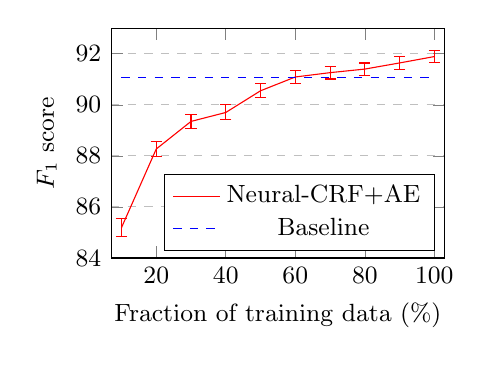
\begin{tikzpicture}
    \tikzstyle{every node}=[font=\small]

  \begin{axis}[
  	xlabel={Fraction of training data (\%)},
  	ylabel={$F_1$ score},
    xmin=7, xmax=103,
    ymin=84, ymax=93,
    height=4.5cm,
    ymajorgrids=true,
    grid style=dashed,
    width=0.48\textwidth,
    legend pos=south east
  ]

  \addplot[color=red, error bars/.cd, y dir=both, y explicit] coordinates {
  (10, 85.19)+=(10, 0.34)-=(10, 0.34)
  (20, 88.27)+=(20, 0.29)-=(20, 0.29)
  (30, 89.35)+=(30, 0.28)-=(30, 0.28)
  (40, 89.70)+=(40, 0.30)-=(40, 0.29)
  (50, 90.55)+=(50, 0.27)-=(50, 0.27)
  (60, 91.09)+=(60, 0.26)-=(60, 0.26)
  (70, 91.26)+=(70, 0.25)-=(70, 0.25)
  (80, 91.40)+=(80, 0.24)-=(80, 0.24)
  (90, 91.64)+=(90, 0.25)-=(90, 0.25)
  (100, 91.89)+=(100, 0.23)-=(100, 0.23)
  };
  \addlegendentry{Neural-CRF+AE}
  \addplot[blue, dashed] coordinates{(10,91.06)(100, 91.06)};
  \addlegendentry{Baseline}
  \end{axis}
\end{tikzpicture}

\vspace{-2ex}
\caption{Comparing the Neural-CRF+AE (red solid line) trained with varying amounts of data vs.\@ a Neural-CRF baseline (blue dashed line), trained on the full training set. Performance averaged over 5 runs, and error bars show $\pm$ 1 std.\@dev.}
\label{figure2}
\end{figure}

Neural systems typically require a large amount of annotated data.
Here we measure the impact of training with varying amount of annotated data,  as shown in  \figref{figure2}.
Wtih the proposed model architecture, the amount of labelled training data can be drastically reduced:
our model, achieves comparable performance against the baseline Neural-CRF, with as little as 60\% of the training data. 
Moreover, as we increase the amount of training text, the performance of Neural-CRF+AE continues to improve.

\paragraph{Hyperparameters}

\begin{figure}[t]

\hspace{-1ex}
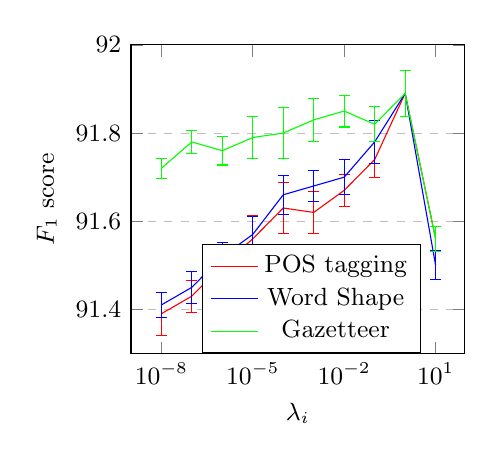
\begin{tikzpicture}
    \tikzstyle{every node}=[font=\small]

  \begin{axis}[
  	xmode=log,
  	xlabel={$\lambda_i$},
  	ylabel={$F_1$ score},
    xmin=0, xmax=90,
    ymin=91.3, ymax=92,
    height=5.5cm,
    ymajorgrids=true,
    grid style=dashed,
    width=0.48\textwidth,
%    legend pos=south east
    legend style={at={(0.87,0)},anchor=south east}
  ]

  \addplot[color=red, error bars/.cd, y dir=both, y explicit] coordinates {
  (1e-8, 91.39)+=(1e-8, 0.0484)-=(1e-8, 0.0484)
  (1e-7, 91.43)+=(1e-7, 0.0361)-=(1e-7, 0.0361)
  (1e-6, 91.50)+=(1e-6, 0.04)-=(1e-6, 0.04)
  (1e-5, 91.56)+=(1e-5, 0.0529)-=(1e-5, 0.0529)
  (1e-4, 91.63)+=(1e-4, 0.0576)-=(1e-4, 0.0576)
  (1e-3, 91.62)+=(1e-3, 0.0484)-=(1e-3, 0.0484)
  (1e-2, 91.67)+=(1e-2, 0.0361)-=(1e-2, 0.0361)
  (1e-1, 91.74)+=(1e-1, 0.04)-=(1e-1, 0.04)
  (1, 91.89)+=(1, 0.0529)-=(1, 0.0529)
  (10, 91.56)+=(10, 0.0289)-=(10, 0.0289)
  };
  \addlegendentry{POS tagging}
  
  \addplot[color=blue, error bars/.cd, y dir=both, y explicit] coordinates {
  (1e-8, 91.41)+=(1e-8, 0.0289)-=(1e-8, 0.0289)
  (1e-7, 91.45)+=(1e-7, 0.0361)-=(1e-7, 0.0361)
  (1e-6, 91.52)+=(1e-6, 0.0324)-=(1e-6, 0.0324)
  (1e-5, 91.57)+=(1e-5, 0.04)-=(1e-5, 0.04)
  (1e-4, 91.66)+=(1e-4, 0.0441)-=(1e-4, 0.0441)
  (1e-3, 91.68)+=(1e-3, 0.0361)-=(1e-3, 0.0361)
  (1e-2, 91.70)+=(1e-2, 0.04)-=(1e-2, 0.04)
  (1e-1, 91.78)+=(1e-1, 0.0484)-=(1e-1, 0.0484)
  (1, 91.89)+=(1, 0.0529)-=(1, 0.0529)
  (10, 91.50)+=(10, 0.0324)-=(10, 0.0324)
  };
  \addlegendentry{Word Shape}
  
  \addplot[color=green, error bars/.cd, y dir=both, y explicit] coordinates {
  (1e-8, 91.72)+=(1e-8, 0.0225)-=(1e-8, 0.0225)
  (1e-7, 91.78)+=(1e-7, 0.0256)-=(1e-7, 0.0256)
  (1e-6, 91.76)+=(1e-6, 0.0324)-=(1e-6, 0.0324)
  (1e-5, 91.79)+=(1e-5, 0.0484)-=(1e-5, 0.0484)
  (1e-4, 91.80)+=(1e-4, 0.0576)-=(1e-4, 0.0576)
  (1e-3, 91.83)+=(1e-3, 0.0484)-=(1e-3, 0.0484)
  (1e-2, 91.85)+=(1e-2, 0.0361)-=(1e-2, 0.0361)
  (1e-1, 91.82)+=(1e-1, 0.04)-=(1e-1, 0.04)
  (1, 91.89)+=(1, 0.0529)-=(1, 0.0529)
  (10, 91.56)+=(10, 0.0289)-=(10, 0.0289)
  };
  \addlegendentry{Gazetteer}
  \end{axis}
\end{tikzpicture}
%}

\vspace{-2ex}
\caption{Effect of hyperparameter values on model performance. Each curve shows the effect of $\lambda_i$, for feature type $i$, with all other $\lambda_j=1, ~j \ne i$. Performance averaged over 5 runs, and error bars show $\pm$ 1 variance.}
\label{figure3}
\end{figure}

Three extra hyperparameters are introduced into our model, controlling the weight of the autoencoder loss relative to the CRF loss, for each feature type.
\figref{figure3} shows the effect of each hyperparameter on test performance. 
Observe that setting $\lambda_i=1$ gives strong performance, and that the impact of the gazetteer is less marked than the other two feature types. 
While increasing $\lambda$ is mostly beneficial, performance drops if the $\lambda s$ are overly large, that is, the auto-encoder loss overwhelms the main prediction task.

\section{Conclusion}\label{sec:conclusion}
%\vspace{-.1in}
In this work, we apply the attentional encoder-decoder for the task of abstractive summarization with very promising results, outperforming state-of-the-art results significantly on two different datasets. Each of our proposed novel models addresses a specific problem in abstractive summarization, yielding further improvement in performance. We also propose a new dataset for multi-sentence summarization and establish benchmark numbers on it. As part of our future work, we plan to focus our efforts on this data and build more robust models for summaries consisting of multiple sentences.


%Our results strongly demonstrate that sequence-to-sequence models are extremely promising for summarization. Some of the other lessons we learned from our experiments are: (i) the LVT-trick is very useful for summarization as it improves training speed while not sacrificing performance; (ii) traditional methods such as vocabulary expansion and syntax-based features can boost performance of deep learning based models as well. As part of our ongoing work, we are investigating on ways to effectively generate rare words in the summary, which appears to be a glaring weakness in the existing models.  


\bibliographystyle{acl_natbib_nourl}
\bibliography{refer}


\end{document}
